\documentclass[11pt]{scrartcl}

\title{Anforderungsspezifikation}
\author{Silvan Adrian \\ Fabian Binna}
\date{\today{}}

\usepackage[ngerman]{babel}
\usepackage[automark]{scrpage2}
\usepackage[colorlinks = true,
linkcolor = black]{hyperref}
\usepackage{color}
\usepackage[normalem]{ulem}
\usepackage{scrpage2}
\usepackage{graphicx}
\usepackage{tabularx}
\usepackage{longtable, tabu}
\graphicspath{ {../22_Grafiken/01_Logo/}{images/}{../../22_Grafiken/01_Logo/} }
\pagestyle{scrheadings}

\clearscrheadfoot
\ihead{
\includegraphics[scale=0.3]{SDDC}}
\ohead{Projekt: SDDC}
\ifoot{Template}
\cfoot{Version: 1.03}
\ofoot{Datum: \today{}}
\setheadsepline{0.5pt}
\setfootsepline{0.5pt}

\usepackage{ucs}
\usepackage[utf8]{inputenc}
\usepackage[T1]{fontenc}


\begin{document}
\def\arraystretch{1.5}
\begin{titlepage}
\begin{center}
\vspace{10em}

\includegraphics[scale=2]{SDDC}
\vspace{10em}
\end{center}
\begin{center}
\huge {Anforderungsspezifikation}
\end{center}
\begin{center}
\vspace{10em}
\LARGE {Silvan Adrian} \\
\LARGE {Fabian Binna}
\end{center}

\end{titlepage}

\newpage
\section{Änderungshistorie}
\begin{tabularx}{\linewidth}{l l X l}
\textbf{Datum} & \textbf{Version} & \textbf{Änderung}  & \textbf{Autor} \\
\hline
\textbf{02.10.15} & 1.00 & Erstellung des Dokuments & Gruppe \\
\textbf{02.10.15} & 1.01 & Nicht funktionale Anforderungen & Silvan Adrian\\
\textbf{02.10.15} & 1.02 & Use Cases Aktoren + User Stories Aktoren & Silvan 
Adrian\\
\textbf{03.10.15} & 1.03 & Anforderungen API & Fabian Binna\\

\end{tabularx}

\newpage
\tableofcontents
\newpage

\section{Einführung}
\subsection{Zweck}
Dieses Dokument beinhaltet die Anforderung zur Analyse.
\subsection{Gültigkeitsbereich}
Dieses Dokument ist während des ganzen Projekts gültig.


\subsection{Referenzen}
-

\section{Anforderungen}
\subsection{API}
Die API definiert einen Workflow der einen Service auf einer Cloud erstellt. Es ist offen, ob dieser Service über mehrere Cloud Anbieter hinaus geht. Der Service wird durch ein Konfigurationsfile (z.B. json) definiert. Zusätzlich können Scriptfiles referenziert werden, die die Software auf den Instanzen installieren. Ein Service kann auch wieder gelöscht werden. Es ist nicht die Aufgabe der API existierende Services zu identifizieren. Die API muss Modular sein, das heisst es sollte möglich sein andere oder eigene Programme für die Cloud Kommunikation zu verwenden. Innerhalb der API werden Compute, Storage, Network usw. als ServiceModule bezeichnet. Diese Abstraktion ermöglicht das wiederverwerten und erweitern der API.

\subsection{Dashboard}

\section{Use Cases}
\subsection{Use Case Diagramm}
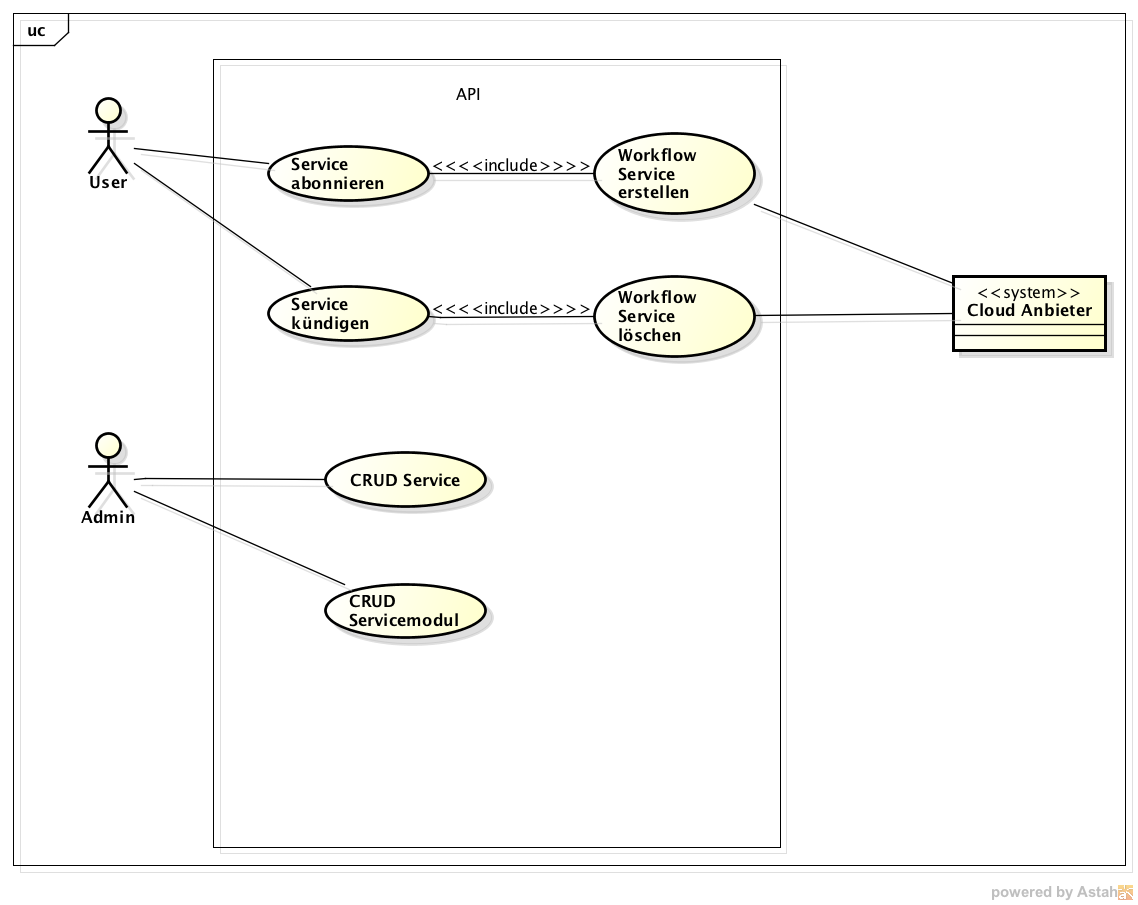
\includegraphics[width=\textwidth]{UseCase-Diagramm}
\subsection{Aktoren \& Stakeholders}
\subsubsection{User}
Als User möchte ich meine abonnierten Services verwalten.
\\
\begin{tabularx}{\linewidth}{l l X }
  \textbf{Aktor} & \textbf{Typ} & \textbf{Ziele}\\
  \hline
  User & Primary & 
  \begin{minipage}{5in}
  \vskip 4pt
  \begin{itemize}
    \item Service abonnieren
    \item Service kündigen
  \end{itemize}
  \vskip 4pt
 \end{minipage}\\
 \hline
\end{tabularx}


\subsubsection{Admin}
Als Admin möchte ich Services und Servicemodule verwalten können.
\\
\begin{tabularx}{\linewidth}{l l X }
  \textbf{Aktor} & \textbf{Typ} & \textbf{Ziele}\\
  \hline
  Admin & Primary & 
  \begin{minipage}{5in}
  \vskip 4pt
  \begin{itemize}
    \item Service erstellen
    \item Service anpassen
    \item Service löschen
    \item Servicemodul erstellen
    \item Servicemodul anpassen
    \item Servicemodul löschen
  \end{itemize}
  \vskip 4pt
 \end{minipage}\\
 \hline
\end{tabularx}


\subsection{Beschreibungen fully dressed}
\subsubsection{Service abonnieren}
\begin{longtabu} to \textwidth {X[1,l] X[2,l]}
	\bfseries Primäraktor & User  \\\hline 
	\bfseries Steakholders und Interessen & Spieler: Möchte einen Service abonnieren  \\\hline 
	\bfseries Vorbedingungen & Das User-Dashboard wurde geöffnet  \\\hline 
	\bfseries Nachbedingungen & Das User-Dashboard wurde geschlossen  \\\hline 
	\bfseries Standartablauf & 
		\begin{enumerate}
			\item Der User gibt die Webadresse für das Dashboard ein
			
		\end{enumerate}
      \\\hline
	\bfseries Spezielle Anforderungen & siehe nichtfunktionale Anforderungen  \\\hline 
	\bfseries Technologie- und Datenvarianten & Keine  \\\hline 
	\bfseries Auftrittshäufigkeit & mehrmals pro Woche  \\\hline 
	\bfseries Offene Fragen & Keine  \\\hline  
\end{longtabu}


\section{User Stories}
\subsection{Rollen}
\subsubsection{User}
Als User benutze ich das Dashboard, um mir einen Service zu abonnieren und 
\subsubsection{Admin}
Als Admin benutze ich die API über die Kommandozeile oder nutze das 
Admin-Dashboard um neue Services zusammenzustellen.



\section{Nichtfunktionale Anforderungen}
\subsection{Menge}
\begin{itemize}
  \item Die Software unterstützt mehr als 30 Cloud Anbieter (libcloud)
  \item Bei jedem Cloud Anbieter bestehen eine gewisse Anzahl Services (von Anbieter zu Anbieter verschieden)
\end{itemize}

\subsection{Schnittstellen}
\begin{itemize}
  \item Die Software wird über HTTP/HTTPS angesprochen
  \item Zur Interaktion im Admin-Dashboard werden die herkömmlichen 
  Schnittstellen gebraucht (Maus,Tastatur,Bildschirm)
  \item Interaktionen können auch über die Kommandozeile ausgeführt werden
\end{itemize}
\subsection{Qualitätsmerkmale}
\subsubsection{Funktionalität}
siehe Abschnitt API und Dashboard
\subsubsection{Zuverlässigkeit}
\begin{itemize}
  \item Der Workflow zum erstellen eines Services soll entweder durchgeführt und 
  abgeschlossen werden oder falls Unterbruch/Fehler rückgängig gemacht 
  werden.
  \item Die Software soll verteilt betrieben werden und eine möglichst hohe 
  Verfügbarkeit bieten
\end{itemize}
\subsubsection{Benutzerbarkeit}
\begin{itemize}
  \item Die Software kann über das vorgesehene Admin-Dashboard benutzt werden
  \item Die API kann auch über die Kommandozeile angesprochen werden
\end{itemize}
\subsubsection{Effizienz}
\begin{itemize}
  \item 
\end{itemize}
\subsubsection{Änderbarkeit}
Die Software soll modular aufgebaut werden, damit Erweiterungen in Zukunft 
problemlos möglich sind.
\subsubsection{Übertragbarkeit}
Das Projekt wird in Python geschrieben ist somit also auf Python mindestens in der Version 2.5 angewiesen, 
kann allerdings durch den Einsatz eines Docker Containers einfach Übertragbar 
gemacht werden.
\end{document}